\chapter{Felhasználói dokumentáció} % User guide
\label{ch:user}

% ==========================================================
% |               Ismertetés, célközönség                  |
% ==========================================================
\section{Ismertetés}
Az alkalmazás segítségével vizualizálni tudjuk offline mozgóképes tartalmainkat egy könnyen kezelhető és esztétikus megjelenésű platformon, továbbá képes a filmek és sorozatok külön kezelésére, felismerésére - amennyiben a filmek nevezéke megfelelő -, a beolvasott tartalmak keresésére, lejátszására, megállítására, pörgetésére, felirat választására, meta-adatok letöltésére filmes adatbázisból vagy betöltésére fájlnévből, NFO fájlból, mindemellett lejátszási listák létrehozására.

Az alkalmazás első indításakor még nem fogunk találni semmilyen tartalmat a Fő képernyőn, ehhez ugyanis előszőr be kell importálnunk a tartalmakat. A Source Importer eszközt használva, kiválasztjuk a megfelelő mappákat, ezután a szoftver beolvassa az összes támogatott formátumú fájlt. Ezután ha úgy akarjuk meta-adatokat tudunk letölteni a beolvasott fájlokhoz. Innentől kezdve az alkalmazás minden funkciója készen áll a használatra.

\subsection{Célközönség}
Az alkalmazás célközönségét nem igazán lehet vagy érdemes leszűkítani egy kisseb csoportra, tekintve, mindenkinek szól, aki kicsit is szereti a filmeket, sorozatokat, hozzászokott a különböző streaming szolgáltatók által nyújtott kényelemhez, funkcionalitáshoz és rendelkezik offline média tartalmakkal, legyenek azok akár filmek, akár sorozatok.

% ==========================================================
% |               Rendszerkövetelmények                    |
% ==========================================================
% \cleardoublepage
\section{Rendszerkövetelmények}
\subsection{Hardveres követelmények}
Az alkalmazás futtatásához lényegében egy Google Chrome-ot és Node.JS-t futtatni képes konfigurációra van szükség csupán. Ettől függetlenül ajánlott az alábbi technikai követelmények teljesítése:
\begin{itemize}
    \item {\textbf {Kijelző: }} legalább HD, azaz 1280×720 pixel
	\item {\textbf {Memória: }} legalább 4 GB
	\item {\textbf {Háttértár: }} legalább 200 MB
\end{itemize}

\subsection{Internetkapcsolat}
Az alkalmazás futtatására alapvetően nincs szükség internet kapcsolatra, azonban a teljes élmény és funkcionalitás eléréséhez erősen ajánlott. Például a meta-adatok letöltése online filmes adatbázisból történik, aminek működéséhez elengedhetetlen az internet kapcsolat.

\subsection{Softwares követelmények}
Három előre telepítendő softwarere van szükségünk, amelyek az alkalmazás működéséhez és fejlesztéséhez elengedhetetlenek. Ezek pedig:
\begin{itemize}
	\item Node.JS
	\item Node Package Manager
	\item Yarn Package Manager
\end{itemize}

\subsection{Operációs rendszer}
Az Electron applikációk sajátja, hogy egy kódbázisból - ami jelen esetben HTML, CSS, JavaScript/TypeScript - mindhárom főbb asztali platformra képes teljes funkcionalitású alkalmazást készíteni. Éppen ezért a támogatott operációs rendszerek az alábbiak:
\begin{itemize}
	\item Microsoft Windows
	\item Linux/GNU
	\item MacOS
\end{itemize}

% ==========================================================
% |                 Telepítési útmutató                    |
% ==========================================================
\section{Telepítési útmutató}
Több mód is elérhető az alkalmazás telepítésére. Az egyik lehetséges mód a kódból már Production változattá fordított {\textbf {futtatható állomány}} futtatása, a másik pedig a {\textbf {Yarn}} Package Manager-t felhasználva. Az alábbiakban mindkét módot tárgyalni fogjuk:

\subsection{Telepítés futtatható állománnyal}
Az alkalmazásból létezik telepíthető, futtatható állomány, ehhez semmi másra nincs szükség csupán a telepítő elindítására. A telepítő ekkor kicsomagolja majd feltelepíti az alkalmazást a számítógépre, parancsikont hoz létre az asztalra és automatikusan el is indítja az alkalmazást.

\subsection{Telepítés és futtatás Yarn segítségével}
Először is szükség van a megfelelő szoftverek telepítésére, mégpedig a Node.JS-re, Node Package Manager-re (továbbiakban npm) és a Yarn Package Manager-re (továbbiakban yarn). A Node.JS és az npm letölthető a Node.JS hivatalos oldaláról\cite{node}, amellyel együtt az npm is letölésre kerül, ajánlott továbbá az LTS verzió letölése, amely ``hosszú ideig tartó támogatás''-t jelent. A yarn-t pedig a Yarn hivatalos oldaláról\cite{yarn} érdemes beszerezni.

Ezen szoftverek telepítése után indítható maga az alkalmazás. A projekt leíró, a {\it package.json} fájlban definiált script-ek, amelyekkel az alkalmazást elindítani és lefordítani tudjuk az alábbiak:

\subsubsection{Repository klónozása}
Először is klónoznunk kell a Repository-t, amely a GitHubon található. Ehhez használhatjuk a git clone parancsot - ha telepítve van a gépünkre a Git\cite{git} - vagy le is tölthetjük azt zip formátumban, az élénk zöld ``Code'', majd a ``Download ZIP'' gombra kattintva.
\lstset{caption={Repository klónozása}, label=src:bash}
\begin{lstlisting}[language={Bash}, numbers={none}]
    git clone https://github.com/TMD44/mvp
    cd mvp
\end{lstlisting}

\subsubsection{Függőségek telepítése Yarn segítségével}
Ezután a függőségek telepítése következik, ezek olyan csomagok, modulok amelyek a program futásához (dependencies) vagy fejlesztéséhez (devDependencies) elengedhetelenek.
\lstset{caption={Függőségek telepítése Yarn segítségével}, label=src:bash}
\begin{lstlisting}[language={Bash}, numbers={none}]
    yarn
\end{lstlisting}

\subsubsection{Fejlesztői verzió futtatása}
Innentől kezdve az alkalmazás indítható, buildelhető. Ezzel a paranccsal az alkalmazás egy fejlesztői verziója indítható el, ebben a módban különböző fejlesztői eszközök is elérhetőek, amelyek a produkciós változatba nem kerülnek bele. Például fejlesztői konzol, React és Redux fejlesztői eszköz.
\lstset{caption={Fejlesztői verzió futtatása}, label=src:bash}
\begin{lstlisting}[language={Bash}, numbers={none}]
    yarn start
\end{lstlisting}

\subsubsection{Produkciós verzió futtatása}
Az alábbi paranccsal egy produkciós verzió készíthető el.
\lstset{caption={Produkciós verzió futtatása}, label=src:bash}
\begin{lstlisting}[language={Bash}, numbers={none}]
    yarn build
\end{lstlisting}

\subsubsection{Produkciós verzió létrehozása}
Végül, de nem utolsó sorban az egyik legfontosabb parancs, amellyel az alkalmazás produkciós verziója hozható létre. Ez az utasítás létrehozza magát a telepítő futtatható állományt és egy hordozható állományt, amely telepítés nélküli futtatást tesz lehetővé. Mindezeket a projekt {\it release} mappájába fogjuk találni.

Továbbá a parancshoz különböző kapcsolók társíthatók, amellyel specifikálhatjuk, hogy milyen platformra szeretnénk az alkalmazást buildelni. Az {\it -mwl} kapcsolóval mindhárom platformra tudunk telepítőt létre hozni. (Fontos megjegyezni, hogy MacOS-re csak MacOS-en lehet telepítőt készíteni. Tehát ha például Windowson adjuk ki az -mwl parancsot akkor csak Linuxra és Windowsra tudunk telepítőt készíteni, Macre nem.) A további kapcsolók értelemszerűen specifikusan egy platformra hoznak létre.
\lstset{caption={Produkciós verzió létrehozása}, label=src:bash}
\begin{lstlisting}[language={Bash}, numbers={none}]
    yarn package

    yarn package --[option]
    # All:       -mwl
    # Windows:   --win, -w
    # Linux:     --linux, -l
    # MacOS:     --mac, -m
\end{lstlisting}

% ==========================================================
% |           Program felületek és működésük               |
% ==========================================================
% \cleardoublepage
\section{Program felületek és működésük}

\subsection{Kezdőlap}
\begin{figure}[H]
	\centering
	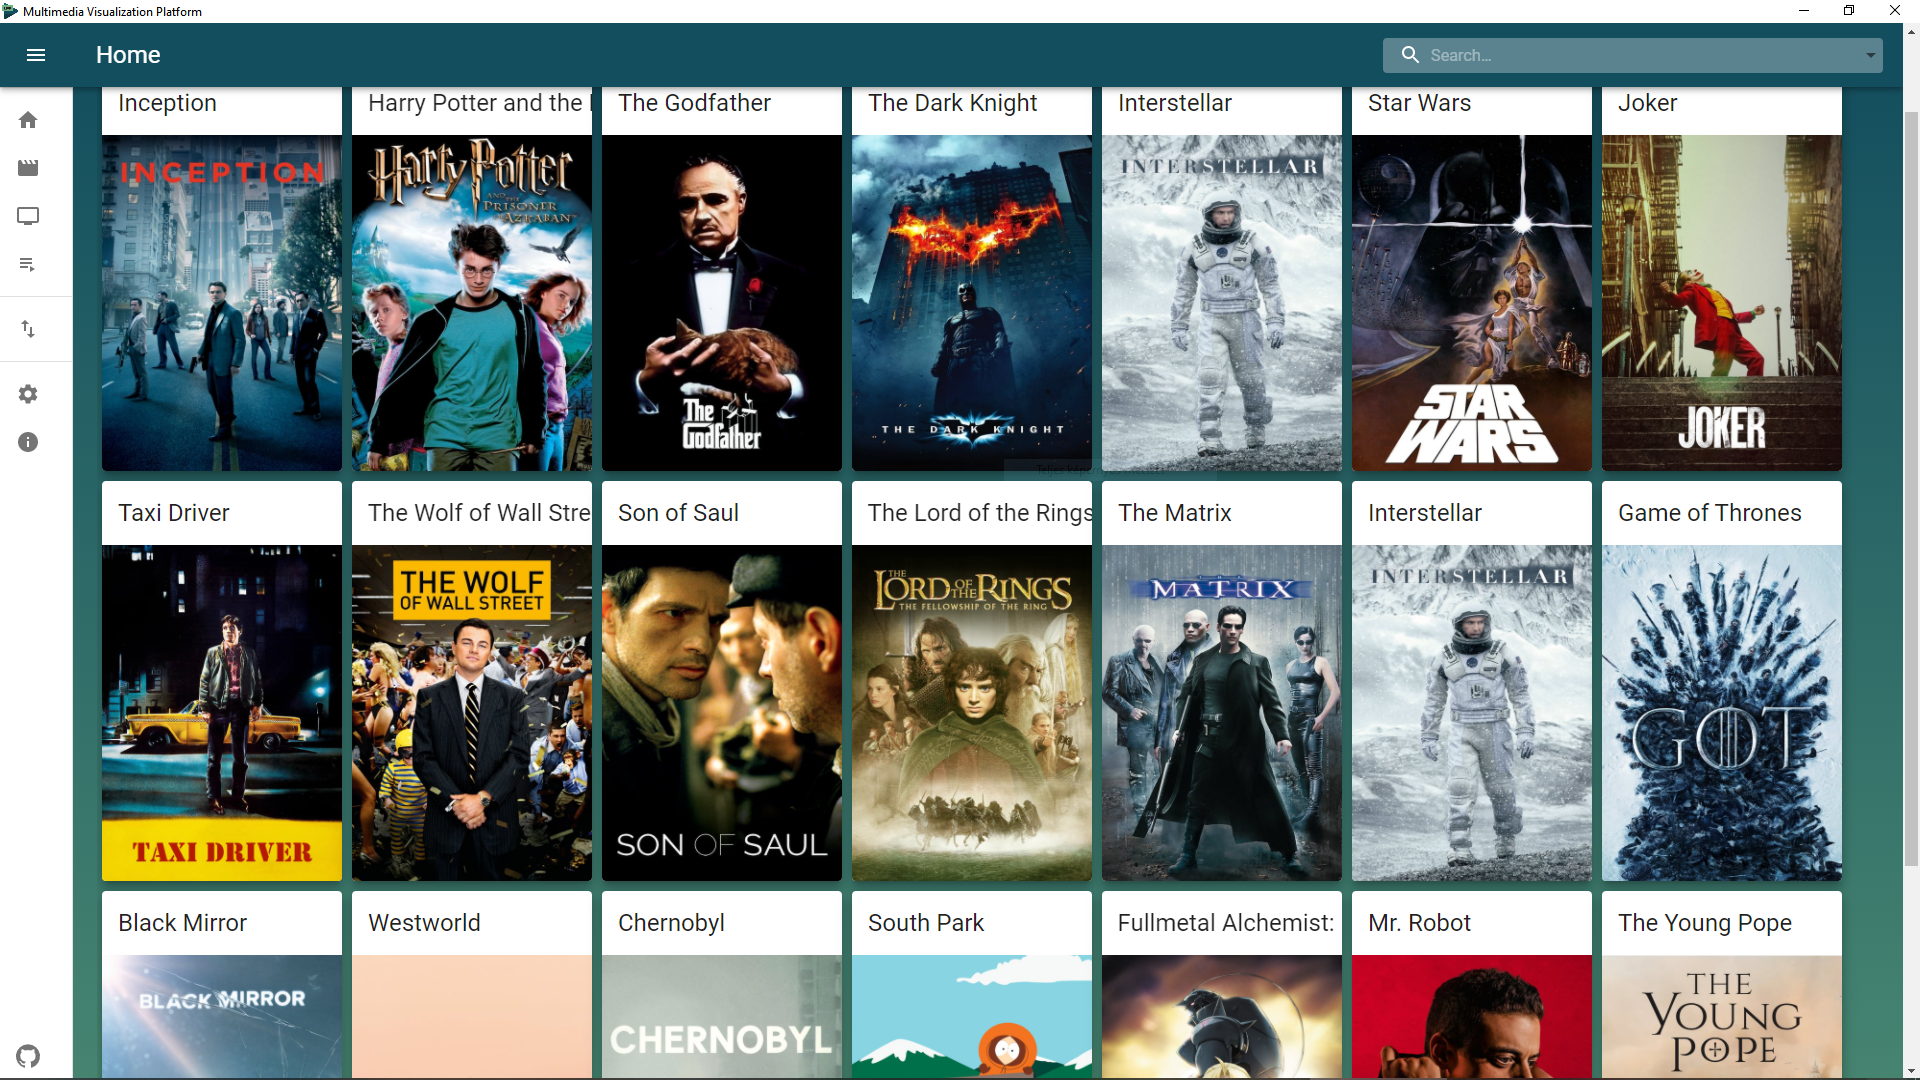
\includegraphics[width=1\textwidth]{home.png}
	\caption{Kezdőlap}
	\label{fig:home}
\end{figure}
A programot elindítva rögtön a Kezdőlapra jutunk, ahol megjelenik az összes beolvasott média tartalom, filmek és sorozatok vegyesen. Ha elsőnek indítjuk el az alkalmazást, akkor a Kezdőlapot üresen fogjuk találni egy üzenettel, hogy még nincs beolvasott média tartalom. Innen a kezdőlapról minden más egyéb oldal könnyen megközelíthető, baloldalt találjuk a Menüt, ahonnan a többi oldalt vagy modalt érjük el. Felül az Alkalmazás sáv kapott helyet, ahol a Menüt vezérlő gomb, a jelenlegi oldal neve és a Kereső sáv található. A média tartalmak alapértelmezetten tízesével jelennek meg az oldalon, ezt azonban van lehetőségünk megváltoztatni: 10, 25, 50 és 100 film/oldalra is. A beolvasott média tartalmak kis kártyákként jelennek meg, melyekre rákattintva a film vagy sorozat adatlapjára oldalára jutunk. Amennyiben a cím túl hosszú a kurzort rávíve a szöveg úszni kezd így elolvashatjuk a teljes címet, továbbá amennyiben nincs az adott filmhez borító kép egy alap minta borító kerül használatra, ezt van lehetőségünk módosítani metadatok letölése funkcióval és kézzel is.

% \cleardoublepage
\subsection{Filmek, Sorozatok}
\begin{figure}[H]
	\centering
	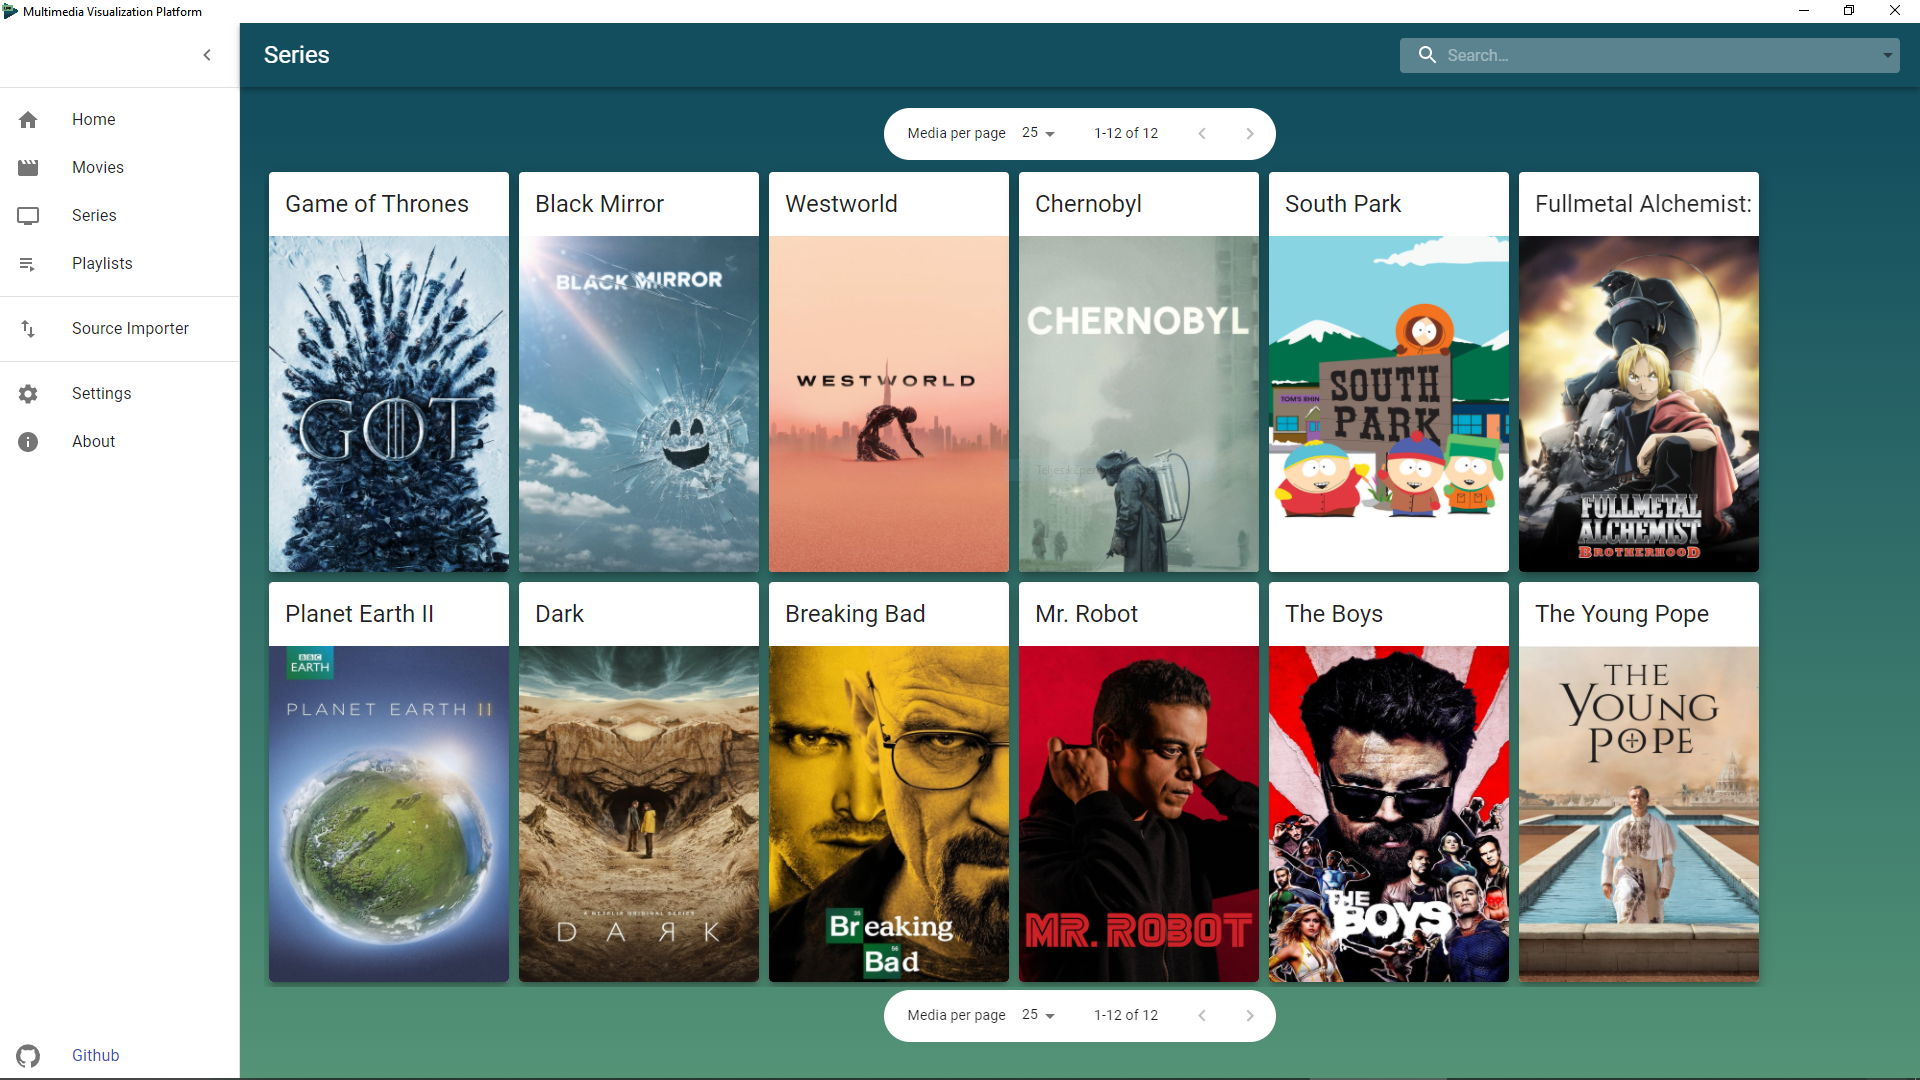
\includegraphics[width=1\textwidth]{movies_series.png}
	\caption{Filmek, Sorozatok}
	\label{fig:movies_series}
\end{figure}
A további oldalakon az alkalmazás tematikusan szétválogatja a beolvasott filmjeinket és sorozatainkat. A 2.4.1-es pontban megfogalmazottak ezekre az oldalakra is érvényesek, tehát az Applikáció struktúrája, baloldalt a Menüsáv, fent az Alkalmazás sáv, Keresés stb. Alapértelmezetten 10 film jelenik meg, ezt a beállítást lehetőségünk van megváltoztatni.

A {\it Filmek} oldalon értelemszerűen a filmeket találjuk.

A {\it Sorozatok} oldalon magától értetődően a sorozatokat. A sorozatok megjelenítése kapcsán, egy kártyát fogunk találni amelyre rákattintva az adatlapon megtaláljuk az összes beolvasott epizódot.

% \cleardoublepage
\subsection{Média adatlap}
\begin{figure}[H]
	\centering
	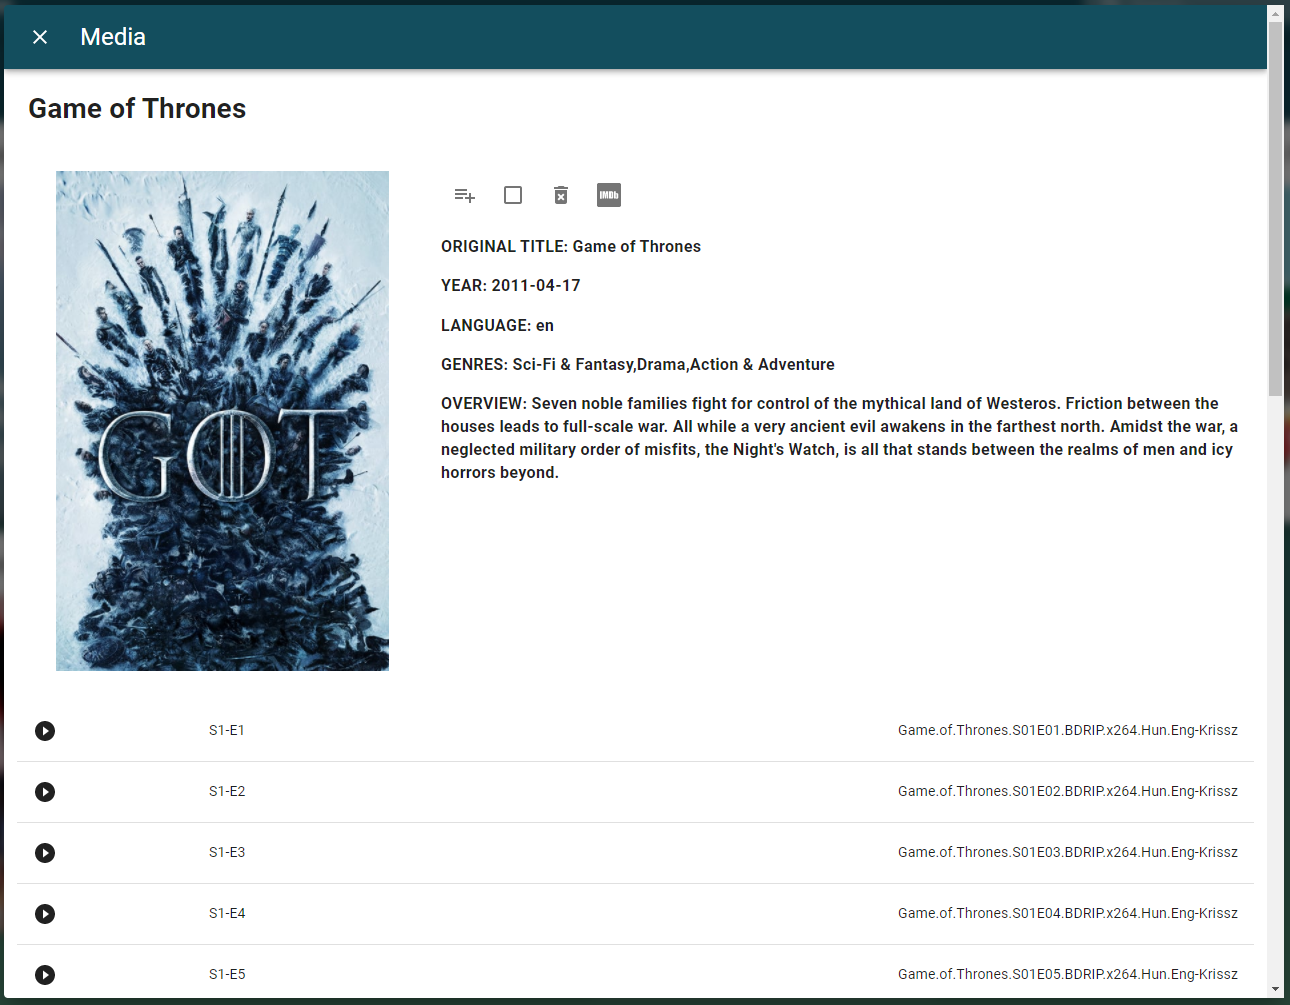
\includegraphics[width=0.9\textwidth]{media_details.png}
	\caption{Filmek, Sorozatok}
	\label{fig:media_details}
\end{figure}
A kiválasztott média kártyájára kattintva megnyílik annak adatlapja, ahol is a fontosabb adatokat - cím, évszám, összefoglalás, borítókép - találjuk, már amennyiben alkalmaztuk az adatbázisból metaadatok letöltése funkciót.

Az adatlapon különböző műveleteket is el tudunk végezni az adott média tartalommal, például törölni tudjuk, ehhez kattintsunk a kuka ikonra - Figyelem, ez a művelet nem visszavonható! - vagy egyedi borítóképet tudunk beállítani ehhez kattintsunk a megfelelő ikonra, abban az esetben ha létezik már borítókép egy üres négyszög alakú ikont találunk, amelyre rákattintva törlődik a jelenlegi borítókép, ekkor az ikon egy kis kép kereső ikonra változik ezzel jelezve, hogy lehetőségünk nyílt új egyedi borítóképet kiválasztani. Megtudjuk nyitni a film IMDB adatlapját, amennyiben a scannelés során a program talált azonosítót, ehhez kattintsunk az IMDB ikonra. Lejátszási listához adásra is itt van lehetőségünk ezt részletesen a 2.4.4-es Lejátszási listák pontban tárgyaljuk.

Ezen az oldalon találjuk továbbá a film elindításához szükséges gombot vagy sorozatok esetén az epizódok elindítása gombokat. Ha a listában rákattintunk valamelyik epizódra vagy filmre, elindul a beépített videólejátszó. A videólejátszóból visszalépni az ESC gomb lenyomásával lehetséges. Az alkalmazás lehetőséget biztosít, hogy továbbra is kedvenc külső videó lejátszó programunkat használjuk a tartalmak lejátszására, ehhez kattintsunk a lista baloldalán elhelyezkedő lejátszás ikonra, ekkor az alkalmazás megnyitja a fájlt az alapértelmezettnek beállított külső lejátszóban.

% \cleardoublepage
\subsection{Lejátszási listák}
\begin{figure}[H]
	\centering
	\subfigure[Lejátszási listák létrehozása]{
		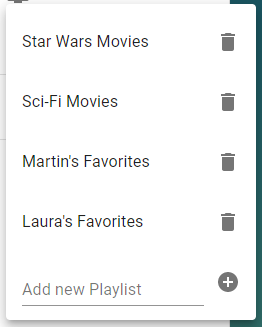
\includegraphics[width=0.35\linewidth]{playlists_1.png}}
	\hspace{5pt}
	\subfigure[Média tartalmak hozzáadása a Lejátszási listához]{
		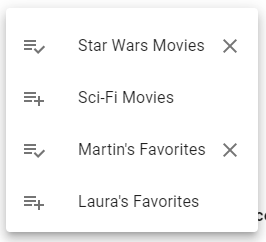
\includegraphics[width=0.35\linewidth]{playlists_2.png}}
	\caption{Lejátszási listák}
	\label{fig:playlists}
\end{figure}
A {\it Lejátszási listák} menüponton belül tudunk hozzáadni új lejátszási listákat, vagy a már létezők között böngészni. Új lejátszási lista hozzáadásához írjuk be a lista nevét, majd nyomjunk Entert vagy kattintsunk a + gombra, ezután a listában megjelenik az általunk hozzáadott elem. Erre rákattintva a főoldalon megjelenik a lejátszási lista tartalma, amennyiben nincs még a listához hozzáadva egy elem sem, azt a felület jelzi számunkra. A teljes lejátszsi listát törölni is tudjuk, a menüpontra kattintva azon belül a jobb oldalon található kuka ikonra kattintva. Ekkor a lista törlődik a rajta lévő filmekkel együtt - fontos megjegyezni, hogy maga a média tartalom nem törlődik a lejátszási lista törlésekor.

Hozzáadni új filmet vagy sorozatot az adott média adatlapján van lehetőségünk. Felül, az ikonsorban kattintsunk a lejátszási lista ikonra, ekkor megnyílik egy kisebb ablak, amelyben a már létrehozott listák találhatók. Kattintsunk a választott listára, ekkor a film hozzáadódik a lejátszási listához, a + jelű ikon, pipás ikonra változik ezzel visszajelezve a felhasználónak, hogy hozzáadódott. Törölni hasonló módon tudunk, ha hozzá van adva a Lejátszási listához egy film, akkor annak adatlapján, a lejátszási listák gombra kattintva, jobb oldalon egy X ikon található, amely megnyomásával a film törlődik a lejátszási listából.

% \cleardoublepage
\subsection{Source Importer}
\begin{figure}[H]
	\centering
	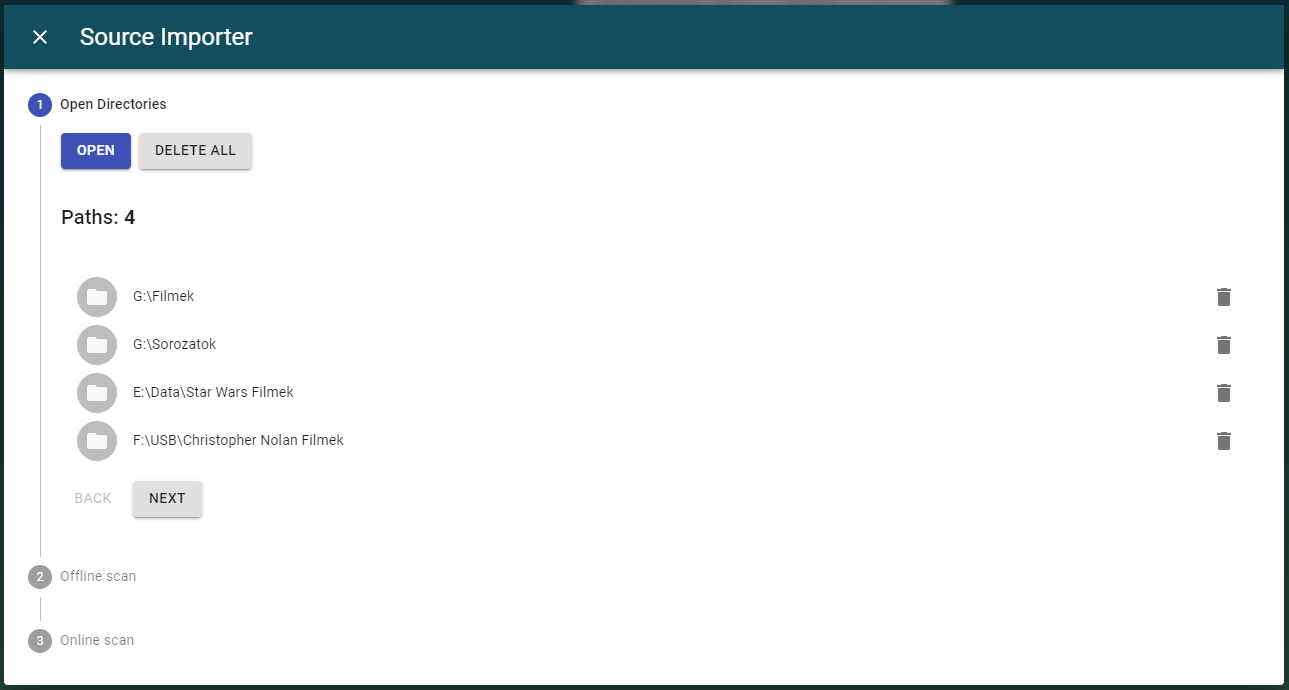
\includegraphics[width=1\textwidth]{source_importer_1.png}
	\caption{Source Importer 1. fázis: Mappa kiválasztás}
	\label{fig:source_importer_1}
\end{figure}
Az alkalmazás egyik legfontosabb része a Source Importer vagy ``forrás importáló''. A Menüben kattintsunk a {\it Source Importer} ikonra ekkor megnyílik a modal ablak, itt tudjuk a média tartalmakat a számítógépünkről vagy adathordozónkról beimportálni az alkalmazásba.

Legelső lépésként ki kell választanunk azokat mappákat ahonnan be szeretnénk a filmeket és sorozatokat importálni. A {\it Mappák megnyitása} gombra kattintva operációs rendszertől függően megnyílik egy párbeszéd ablak, ahol a mappákat ki tudjuk választani, tegyünk így aztán kattintsunk a Mappaválasztás gombra a párbeszéd ablakban. Ekkor visszaérve a Source Importerbe megjelenik a kiválasztott mappák listája, a mappa nevek jobboldalán lévő kis kukára, ha kattintunk egyesével ki tudjuk törölni a kiválasztott elérési útvonalakat, ha pedig az {\it Összes törlése} gombra kattintunk, akkor értelemszerűen az össze mappa törlésre kerül. Ha mindezekkel megvagyunk és a megfelelő mappák vannak kiválasztva kattintsunk a {\it Következő} gombra.

\begin{figure}[H]
	\centering
	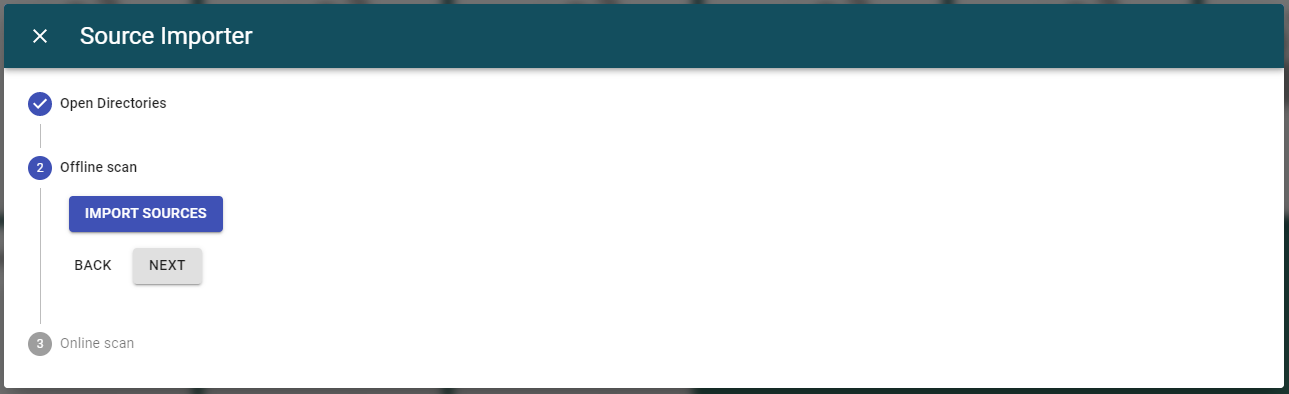
\includegraphics[width=1\textwidth]{source_importer_2.png}
	\caption{Source Importer 2. fázis: Offline scan}
	\label{fig:source_importer_2}
\end{figure}
Az importálási folyamat második állomása az Offline scannelés, kattintsunk a {\it Források importálása} gombra, hogy elinduljon a scannelés. A háttérben a következő dolgok történnek: Az alkalmazás végignézi a kiválasztott mappákat és megkeresi a támogatott formátumú videófájlokat, feliratfájlokat és NFO fájlokat. Sok példa van arra, hogy egy-egy filmfájl mellett minta videófájlok is találhatók, ezeket az alkalmazás szempontjából lényegtelen fájlokat a scannelés során kiszűrjük. Miután megvannak a megfelelő médiafájlok az alkalmazás megpróbál minden használható információt összegyűjteni a fájlnevekből, mappanevekből, NFO fájlokból, majd ezeket összesíti. Például a teljesség igénye nélkül: cím, IMDB ID, felbontás, évszám, nyelv, minőség, évad- és epizódszám, hang és videó kodekek továbbá egyéb hasznos információk.

A scannelés időtartama, ha sok tartalmat importálunk be eltarthat néhány percig.

\begin{figure}[H]
	\centering
	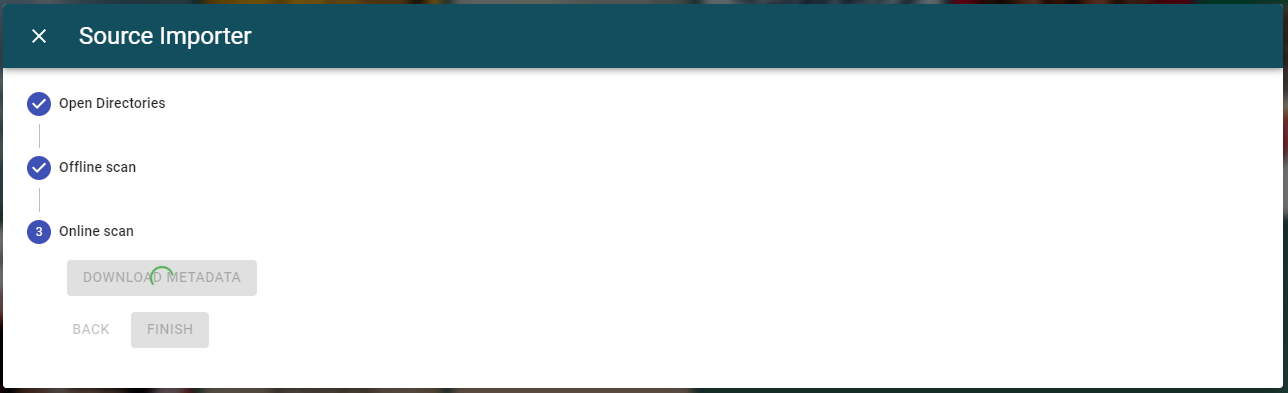
\includegraphics[width=1\textwidth]{source_importer_3.png}
	\caption{Source Importer 3. fázis: Online scan}
	\label{fig:source_importer_3}
\end{figure}
Az importálási folyamat utolsó, harmadik állomása az úgy nevezett Online scannelés, amely gyakorlatilag a meta-adatok letöltését jelenti. Ehhez mint a nevében is benne van internetkapcsolatra lesz szükség, ha ez nincs meg a scannelés nem végződik el. Kattintsuk a {\it Metaadatok letöltése} gombra, ekkor elindul a scannelés.
Ekkor amennyiben az Offline scannelés során talált az alkalmazás IMDB azonosítót - éppen ezért ajánlott ellenőrizni, hogy a média fájlok mellett legyen egy NFO fájl, amely tartalmaz egy helyes IMDB linket, ugyanis ezzel lehet biztosítani azt, hogy ténylegesen a megfelelő adatok kerülnek letöltésre -, úgy ez alapján az azonosító alapján keresi ki a metaadatokat a TMDB adatbázisból majd tölti is le azokat. Amennyiben nem talált azonosítót,úgy ebben az esetben a talált cím és évszám párossal indít keresést. Ez nem száz százalékos bizonyosságal fog jó eredményt visszaadni ugyanis, ha például több film is létezik az adatbázisban hasonló vagy ugyanolyan névvel, vagy ha a fájl nem megfelelő, értelmes módon van elnevezve akkor a név és évszám szerinti keresés hibára vagy eredménytelen válaszra futhat ki.

A scannelés időtartama valamivel több ideig tarthat mint az Offline scannelés, a beolvasott tartalmak és meta-adatok mennyiségétől, az internetkapcsolat gyorsaságától, sávszélesség foglaltságától függően.

% \cleardoublepage
\subsection{Kereső}
\begin{figure}[H]
	\centering
	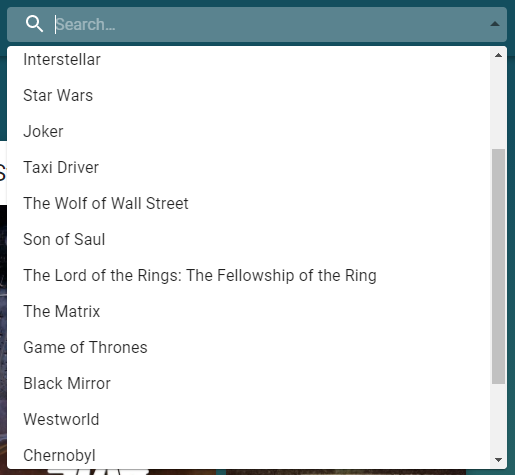
\includegraphics[width=0.6\textwidth]{search.png}
	\caption{Kereső}
	\label{fig:search}
\end{figure}
A fenti Alkalmazás sávon található a Kereső, amely nevére nem rácáfolandón a beolvasott tartalmak közötti keresésre szolgál. Ha rákattintunk a kereső sávra akkor egy legördülő listában azonnal megkapjuk az össze alkalmazás által beolvasott média tartalmat. Szöveges mezőbe írással, pedig ezen a listán tudunk szűkíteni, ha nincs olyan film cím, mint amit beírtunk a kereső jelzi ezt számunkra. Amennyiben megtaláltuk keresett filmünket a legördülő menüben rákattintva megnyílik az adott film vagy sorozat adatlapja, ahol is a fent már részletezett módon lehet eljárni.

% \cleardoublepage
\subsection{Beállítások}
\begin{figure}[H]
	\centering
	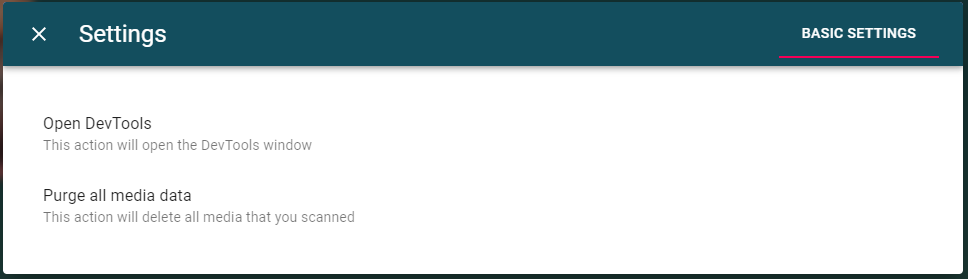
\includegraphics[width=0.8\textwidth]{settings.png}
	\caption{Beállítások}
	\label{fig:settings}
\end{figure}
A Menüben a {\it Beállítások} ikonra kattintva megnyílik a Beállítások ablak, ezen belül az alkalmazás egészére ható fontosabb műveleteket tudjuk elvégezni. Például itt tudjuk teljesen kiüríteni a filmes adatbázisunkat, ez minden beállítást filmet az alapértelmezettre fog visszaállítani. Figyelem, ez a művelet nem visszavonható, minden film, sorozat, ezek metaadatai és a lejátszási listák is törlésre kerülnek!
Innen tudjuk megnyitni a fejlesztői konzolt is.

\subsection{Névjegy}
\begin{figure}[H]
	\centering
	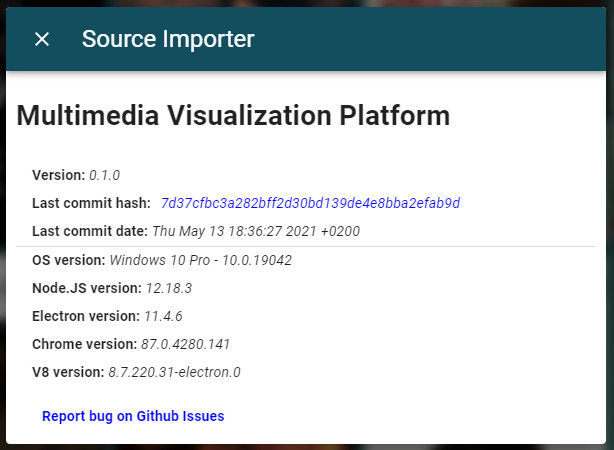
\includegraphics[width=0.7\textwidth]{about.png}
	\caption{Névjegy}
	\label{fig:about}
\end{figure}
A {\it Névjegy} menüponton belül az alkalmazás verziójáról, környezetének verzióiról kapunk hasznos információkat.

% ==========================================================
% |                   Hibaelhárítás                        |
% ==========================================================
% \cleardoublepage
\section{Hibaelhárítás}
Az alkalmazás a fejlesztői konzolon belül jelzi az esetleges hibákat, a konzolt a Beállítások ablakból tudunk megnyitni.

\subsection{``Gyári visszaállítás''}
Bármilyen problémára megoldást nyújthat a ``gyári visszaállítás'', ehhez navigáljunk az alkalmazás telepítési mappájába (Windows esetében, ha a telepítőt használtuk a következő elérési címen találjuk: ``C:/Users/FELHASZNÁLÓ/AppData/Local/Programs/mvp''). A telepítési mappán belül navigáljunk a {\it resources}, majd az {\it assets} mappába, itt a {\it .storage} mappában két JSON fájlt fogunk találni, a {\it config.json} illetve a {\it mediaDB.json} fájlt. Ezen két fájl törlésével vagy a mappából kimozgatásával az alkalmazás eredeti, alapértelmezett állapotába áll vissza.

\subsection{Hibajelzés}
A felmerülő problémák, hibák jelzésére a Github Issues fül ad otthont, amelyet az alábbi címen lehet elérni: \url{https://github.com/TMD44/mvp/issues}

Hibajelzésnél kérjük használja az erre létrehozott sablont, és töltse ki a verzió számokat a {\it Névjegy} oldalról.
